\documentclass{article}

\usepackage[italian]{babel}
\usepackage[letterpaper,top=2cm,bottom=2cm,left=3cm,right=3cm,marginparwidth=1.75cm]{geometry}
\usepackage{amsmath}
\usepackage{graphicx}
\usepackage{subcaption}
\usepackage{textcomp}
\usepackage[colorlinks=true, allcolors=blue]{hyperref}
\usepackage{ragged2e}
\usepackage[dvipsnames]{xcolor}
\usepackage{fancyhdr}

\title{\textbf{Bivacco Casera Pian della Cenere - 1012 metri s.l.m}}
\author{Matteo Drago}

% ==========================================================
% Impostazioni per il logo in ogni pagina
% ==========================================================
\pagestyle{fancy}
\fancyhf{} % Pulisce tutti i campi di intestazione e piè di pagina
\fancyhead[R]{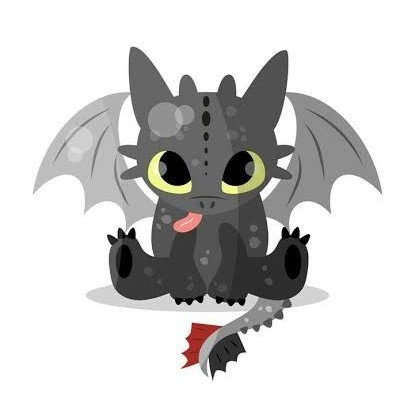
\includegraphics[height=1.5cm]{images/toothless.jpeg}} % Posiziona il logo a destra (R) nell'intestazione
\renewcommand{\headrulewidth}{0pt} % Rimuove la linea orizzontale nell'intestazione (opzionale)


\begin{document}
\maketitle
\thispagestyle{fancy} % Aggiungi questa riga

\begin{abstract}
Questo documento raccoglie e organizza le informazioni che ho acquisito nel corso degli anni sui bivacchi, basate sulle mie esperienze dirette. Sebbene non si proponga come una guida esaustiva e perfetta, offre il minimo indispensabile per una buona vita in bivacco, con consigli pratici e diretti per chiunque desideri affrontare al meglio queste pazze ma piacevoli avventure.
\end{abstract}

\section{Il bivacco}

% ==========================================================
% Immagine a sinistra, testo a destra allineato in alto
% ==========================================================
\noindent
\begin{minipage}[t]{0.45\textwidth}
  \vspace{0pt} % forza l'allineamento in alto
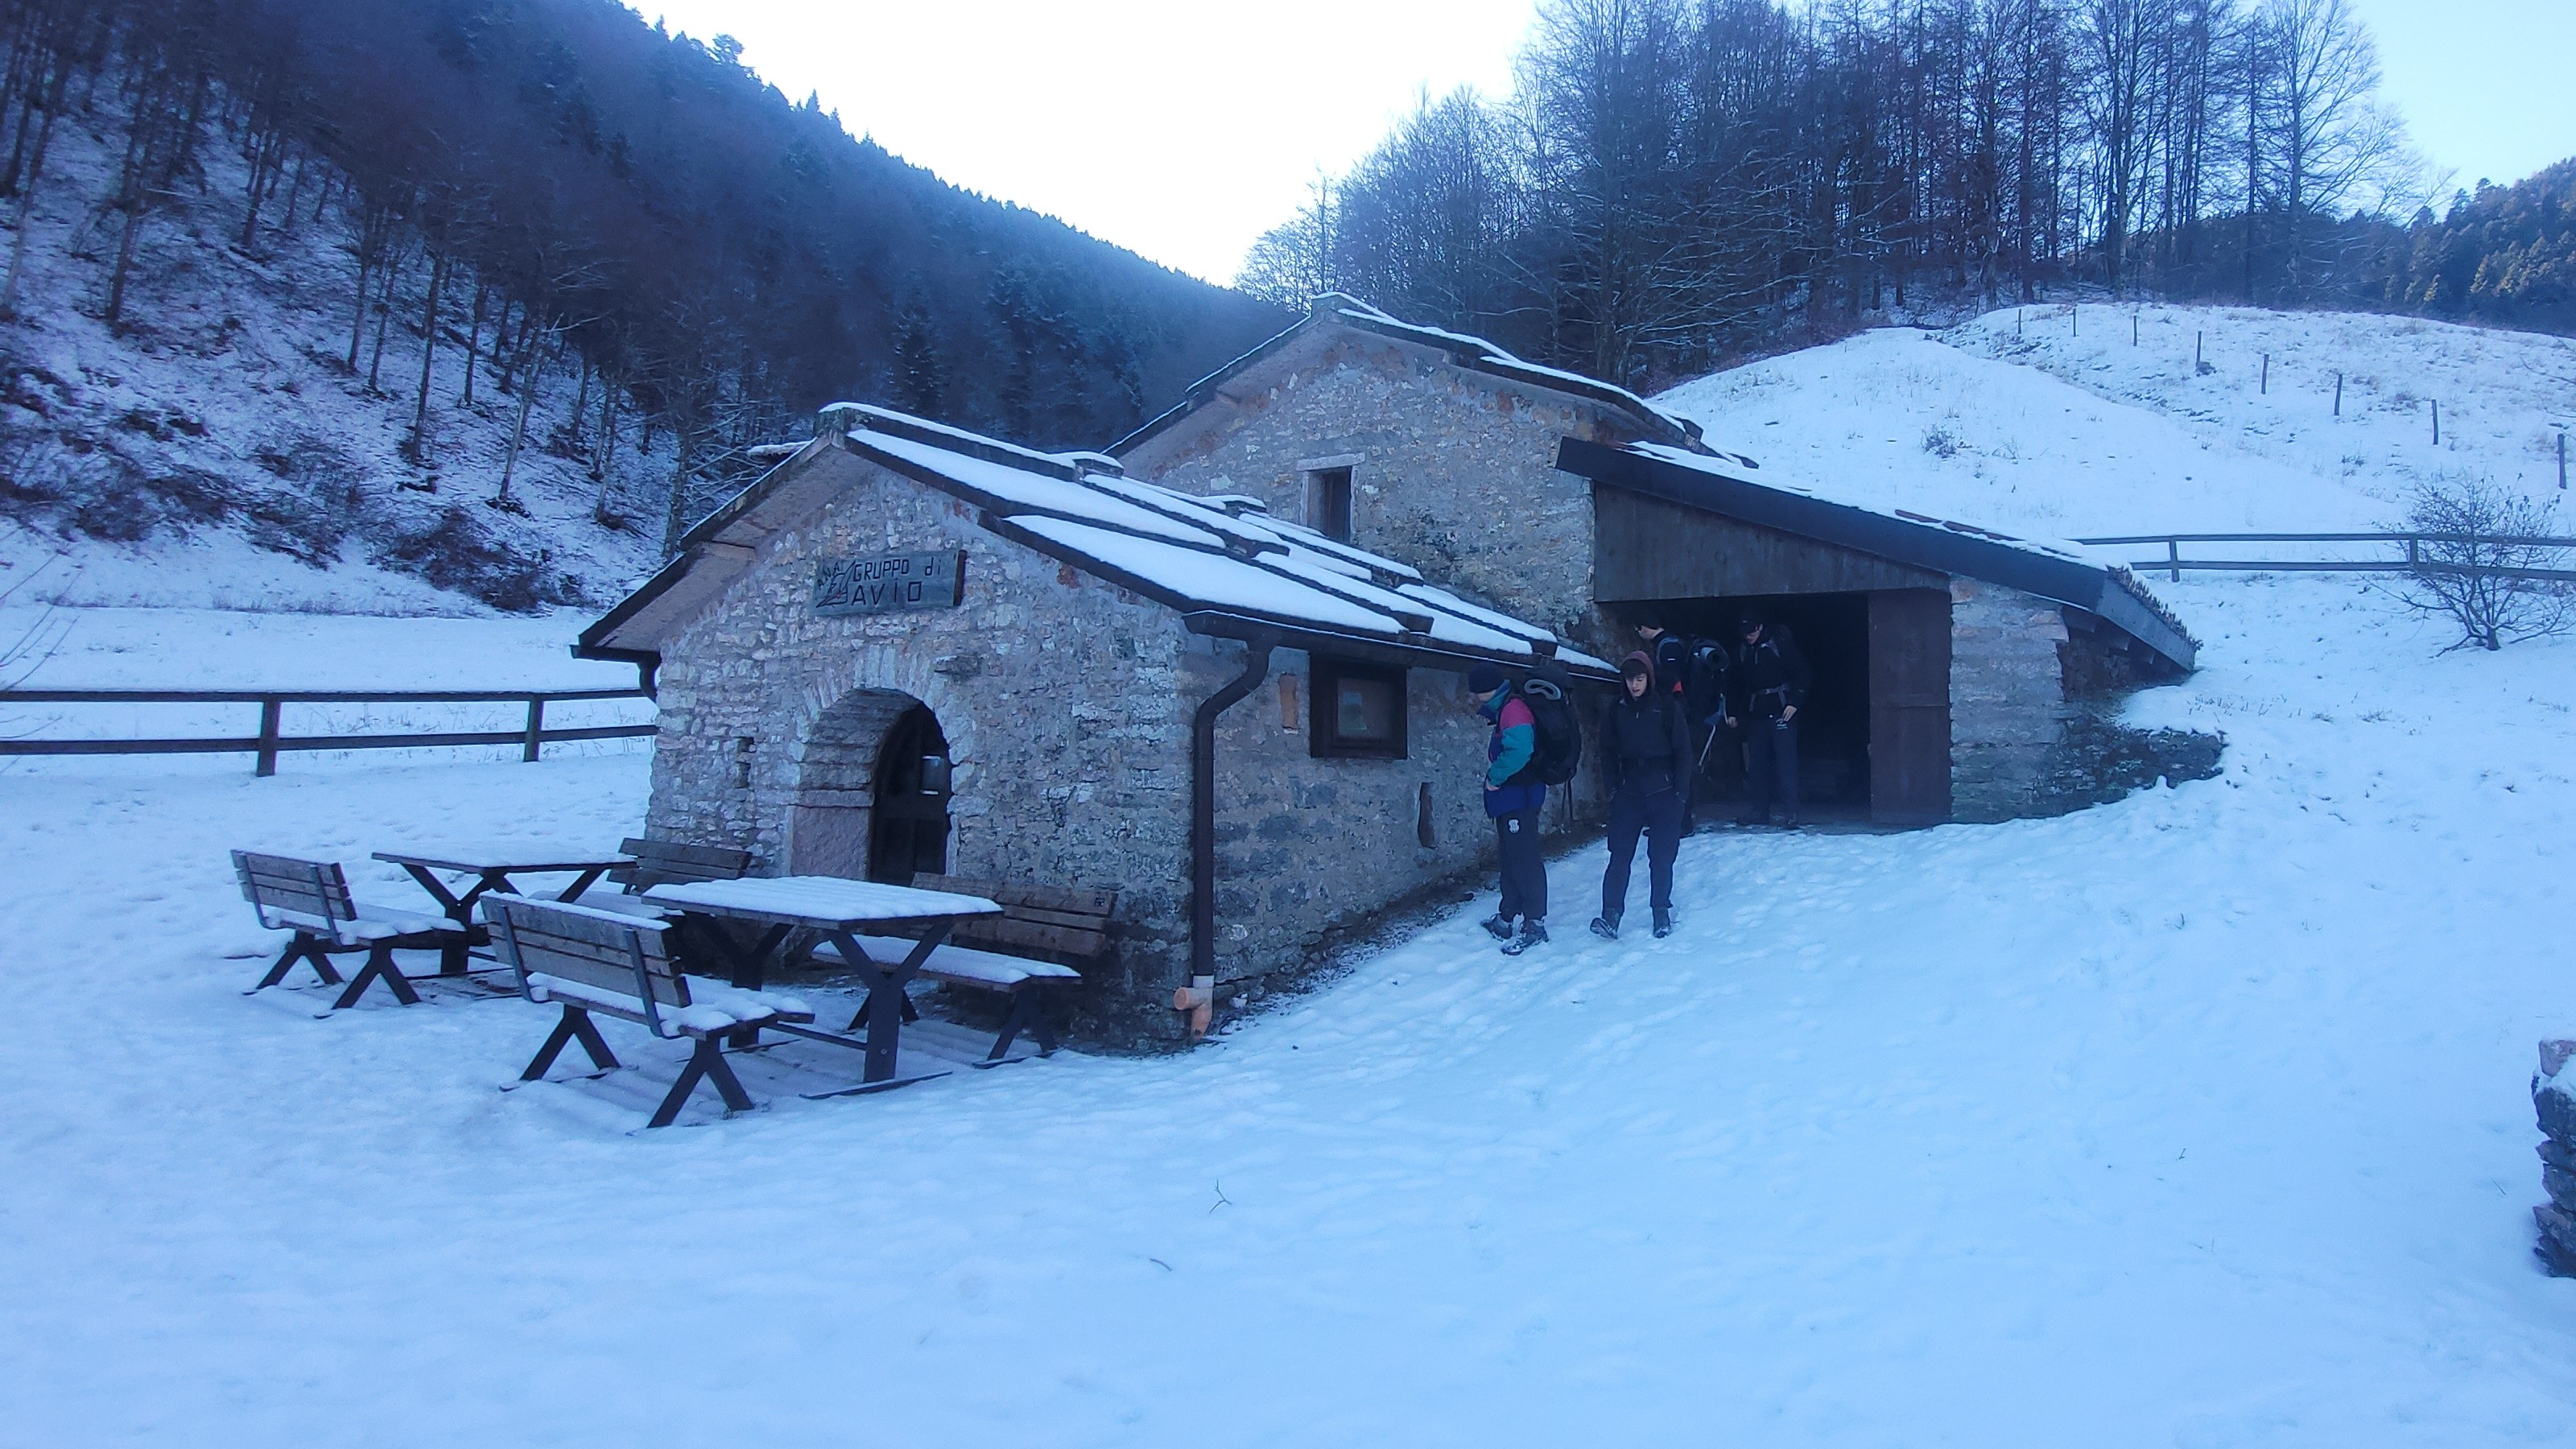
\includegraphics[width=\linewidth,height=8cm,keepaspectratio]{images/bivacco.jpg}
\end{minipage}%
\hfill
\begin{minipage}[t]{0.5\textwidth}
  \vspace{0pt} % forza l'allineamento in alto
  
  Gruppo montuoso\\
  \textbf{\large Monte Baldo}
  \\[1em] % Aggiunge una riga vuota qui
  Località\\
  \textbf{\large Pian della Cenere}
  \\[1em] % Aggiunge una riga vuota qui
  Comune\\  
  \textbf{\large Avio}
  \\[1em] % Aggiunge una riga vuota qui
  Altezza\\  
  \textbf{\large 1012 m s.l.m.}
  \\[1em] % Aggiunge una riga vuota qui
  Apertura\\  
  \textbf{\large Non gestito, sempre aperto}

\end{minipage}

\subsection{Caratteristiche}
Il bivacco Pian della Cenere (ex-Casera) si trova a 1.012 metri, è un posto di ricovero in casi di emergenza o riparo da temporali. L'interno è molto spartano ed essenziale, è presente un camino per riscaldare l'ambiente attrezzato di panche di legno sulle quali si può dormire.
 
Il bivacco è recintato ed è costituito da 2 stanze principali
\begin{itemize}
    \item \textbf{Prima stanza}: più piccola con l'essenziale per "vivere", quindi farsi da mangiare e riscaldarsi, qui si trova un camino molto ampio e 2 tavoli oltre che una piccola dispensa con l'essenziale in caso di emergenza.
    \item \textbf{Seconda stanza}: è molto più grande della precedente, si presentano diversi tavoli e "brande" in legno per mangiare o dormire in compagnia. \textbf{\textcolor{OrangeRed}{(Non ottimale dormire in inverno in quanto la mancanza del camino nella seconda stanza la rende molto fredda, in caso ci si può stringere molto nella prima).}}
    \item \textbf{Spazio esterno}: si presentano due tavolini con panche vicino all'entrata e una "stanza aperta" adibita a legnaia (noi l'abbiamo utilizzata per attaccarci le amache e dormire dal momento che il bivacco era pieno.
\end{itemize}

Non sono presenti fonti d'acqua potabile, vicino all'entrata si trova un abbeveratorio per le mucche ma onestamente lo sconsiglio

Ricavare la legna non è complesso dal momento che il bivacco è circondato dal bosco.

\section{Come ci siamo arrivati}
\subsection{Giro 1}
Abbiamo trovato il bivacco mentre terminavamo il giro del bivacco malga-Lavacchio, è quindi possibile raggiungerlo percorrendo gli stessi sentieri.

\subsection{Giro 2}
In prossimità della casera si trova la Via Ferrata Gerardo Sega, un itinerario di livello intermedio situato nella Valle dei Mulini, con cenge esposte e tratti nel bosco che conducono al Monte Coalaz. Tuttavia causa maltempo non siamo riusciti a percorrerlo. È possibile raggiungere il bivacco anche in macchina, parcheggiando vicino alla malga che si erge vicino al bivacco.


\begin{figure}[htbp!]
    \centering
    % Colonna di sinistra, allineata in alto
    \begin{subfigure}[t]{0.45\textwidth}
        \centering
        \vspace{0pt} % Forziamo l'allineamento in alto
        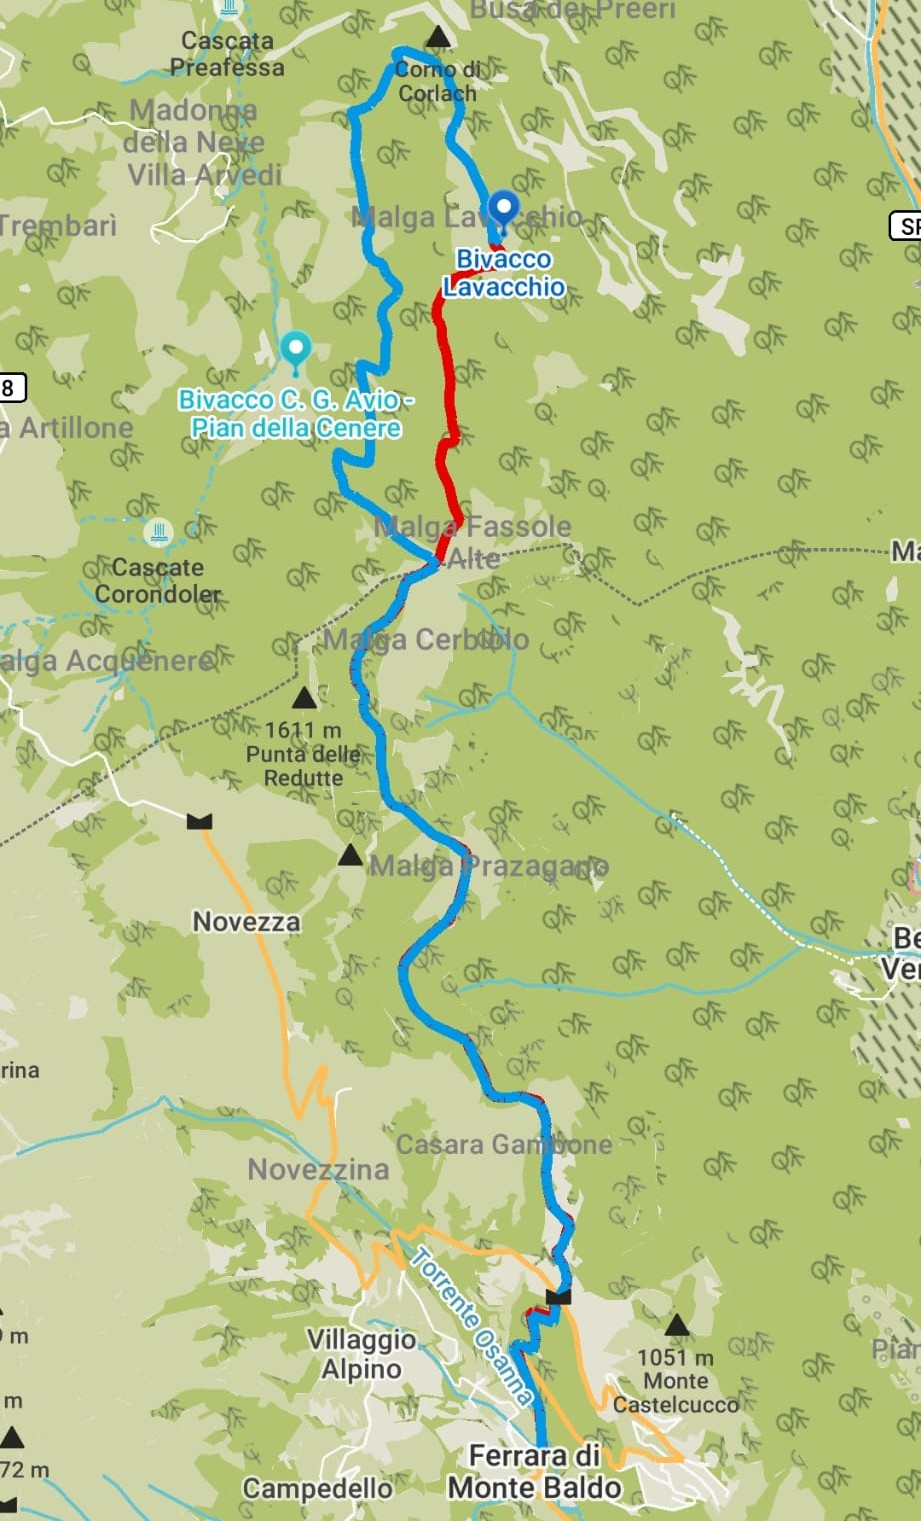
\includegraphics[width=\textwidth]{images/sentiero_mapsMe.jpg}
        \caption{Sentiero su Maps.Me.}
        \label{fig:foto_lunga}
    \end{subfigure}
    \hfill
    % Colonna di destra, allineata in alto
    \begin{subfigure}[t]{0.45\textwidth}
        \centering
        \vspace{0pt} % Forziamo l'allineamento in alto anche qui
        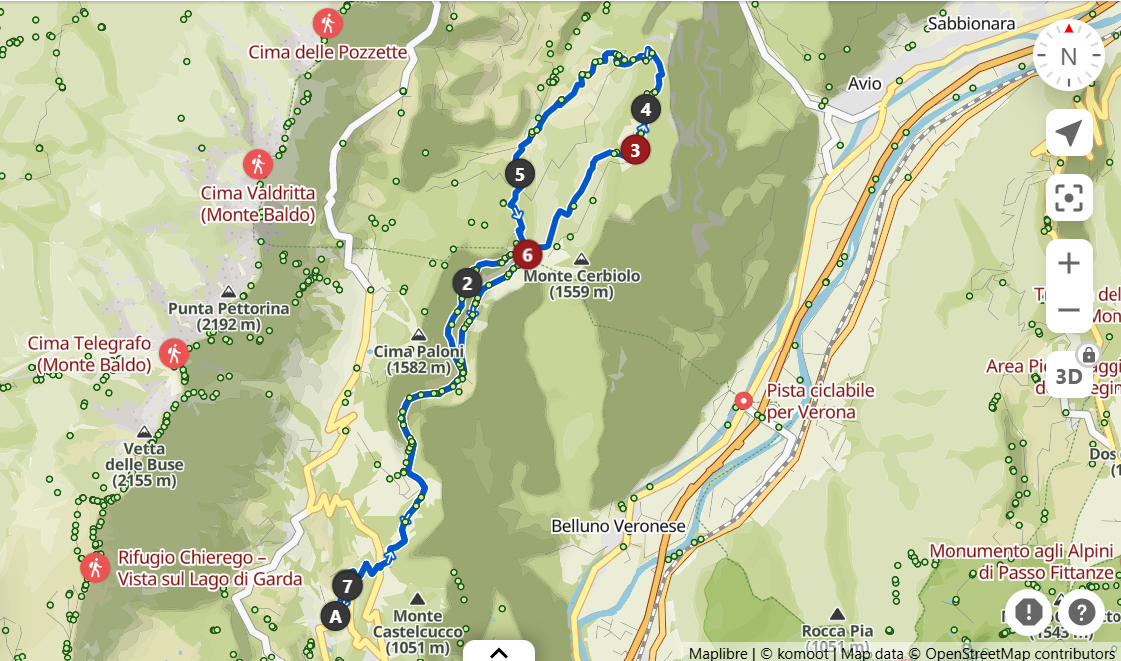
\includegraphics[width=\textwidth]{images/sentiero_komoot.png}
        \caption{Sentiero su Komoot.}
        \label{fig:foto_corta1}
        \vspace{1em} % Aggiunge un po' di spazio tra le due foto
        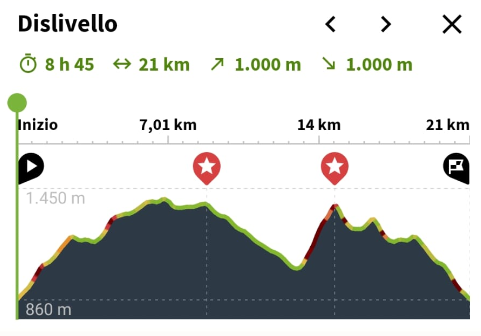
\includegraphics[width=\textwidth]{images/profilo_altimetrico.png}
        \caption{Profilo altimetrico del percorso.}
        \label{fig:foto_corta2}
    \end{subfigure}
    % Didascalia generale per l'intera figura
    \caption{Il sentiero e i dettagli del percorso.}
    \label{fig:panoramica_dettagli}
\end{figure}


\section{Non ti scordar di me}
\textbf{\textcolor{BurntOrange}{Ricorda: il bivacco è un bene comune. Il suo futuro dipende dal rispetto e dal senso civico dei visitatori. Usalo con cura e lascialo più pulito di come l'hai trovato.}}


\section{Alcune foto}

\begin{figure}[htbp!]
    \centering
    % Prima riga: Due foto affiancate
    \begin{subfigure}{0.45\textwidth}
        \centering
        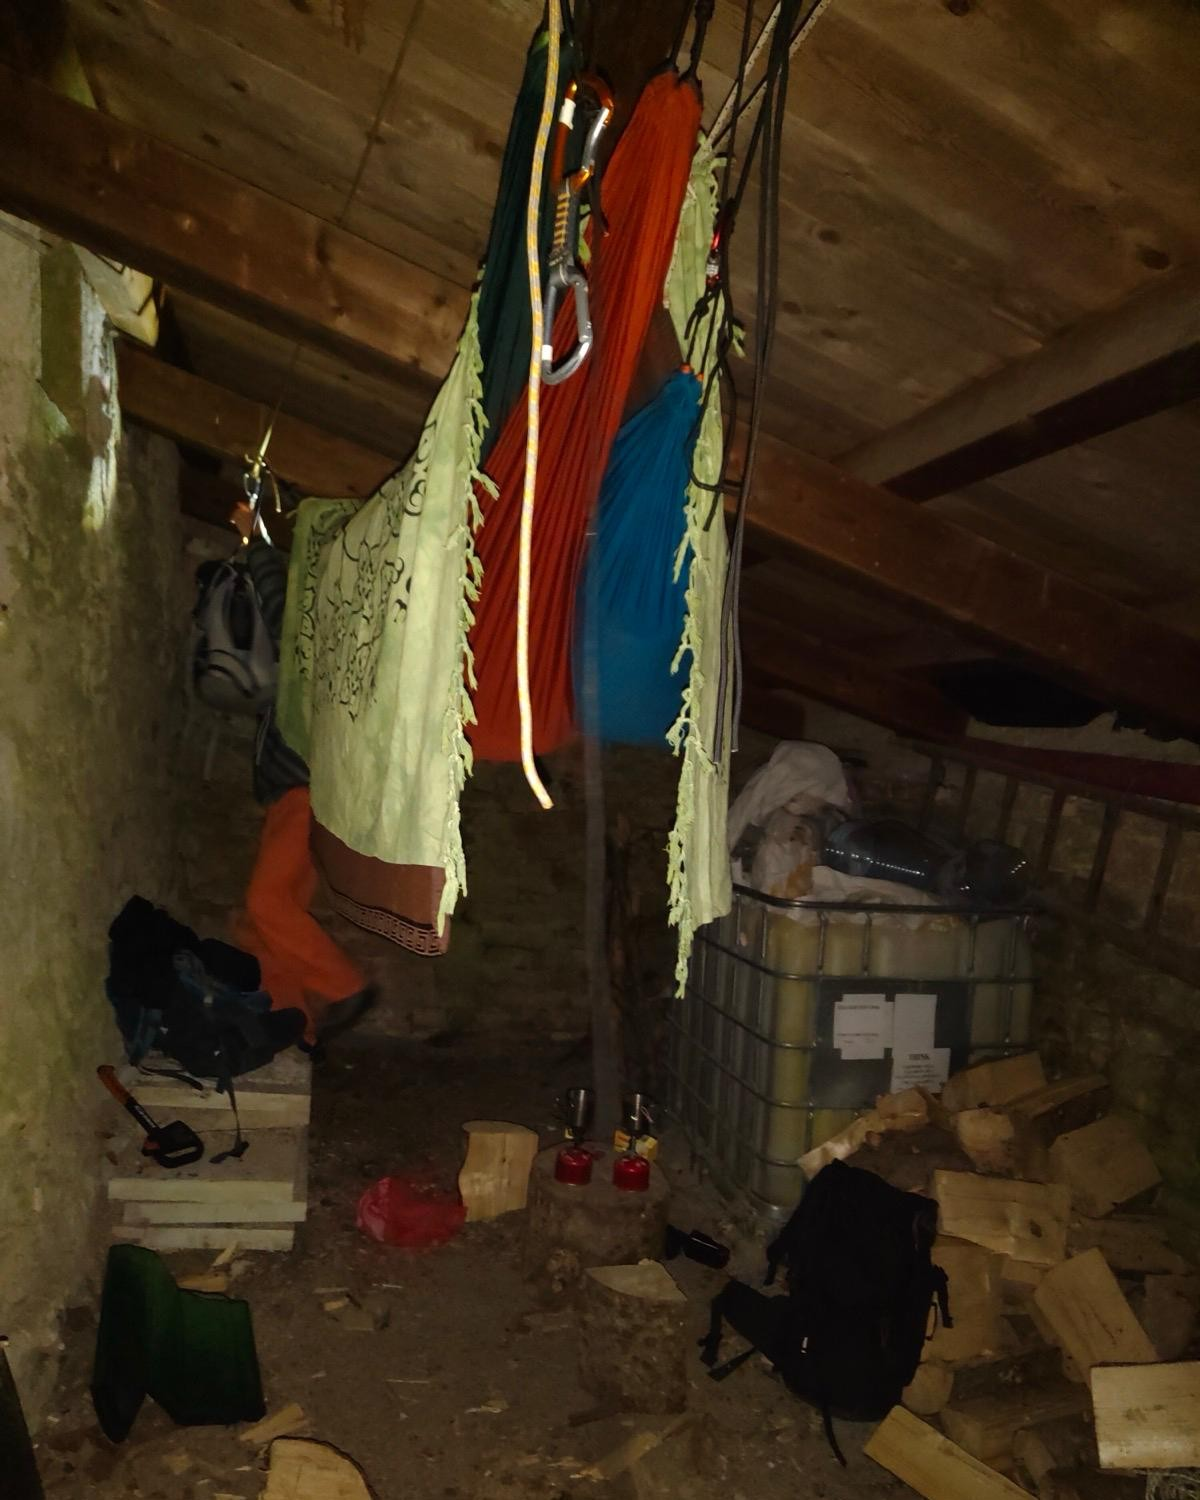
\includegraphics[width=\linewidth]{images/foto_amache.jpg}
        \caption{Notte in amaca.}
        \label{fig:foto1}
    \end{subfigure}
    \hfill 
    \begin{subfigure}{0.45\textwidth}
        \centering
        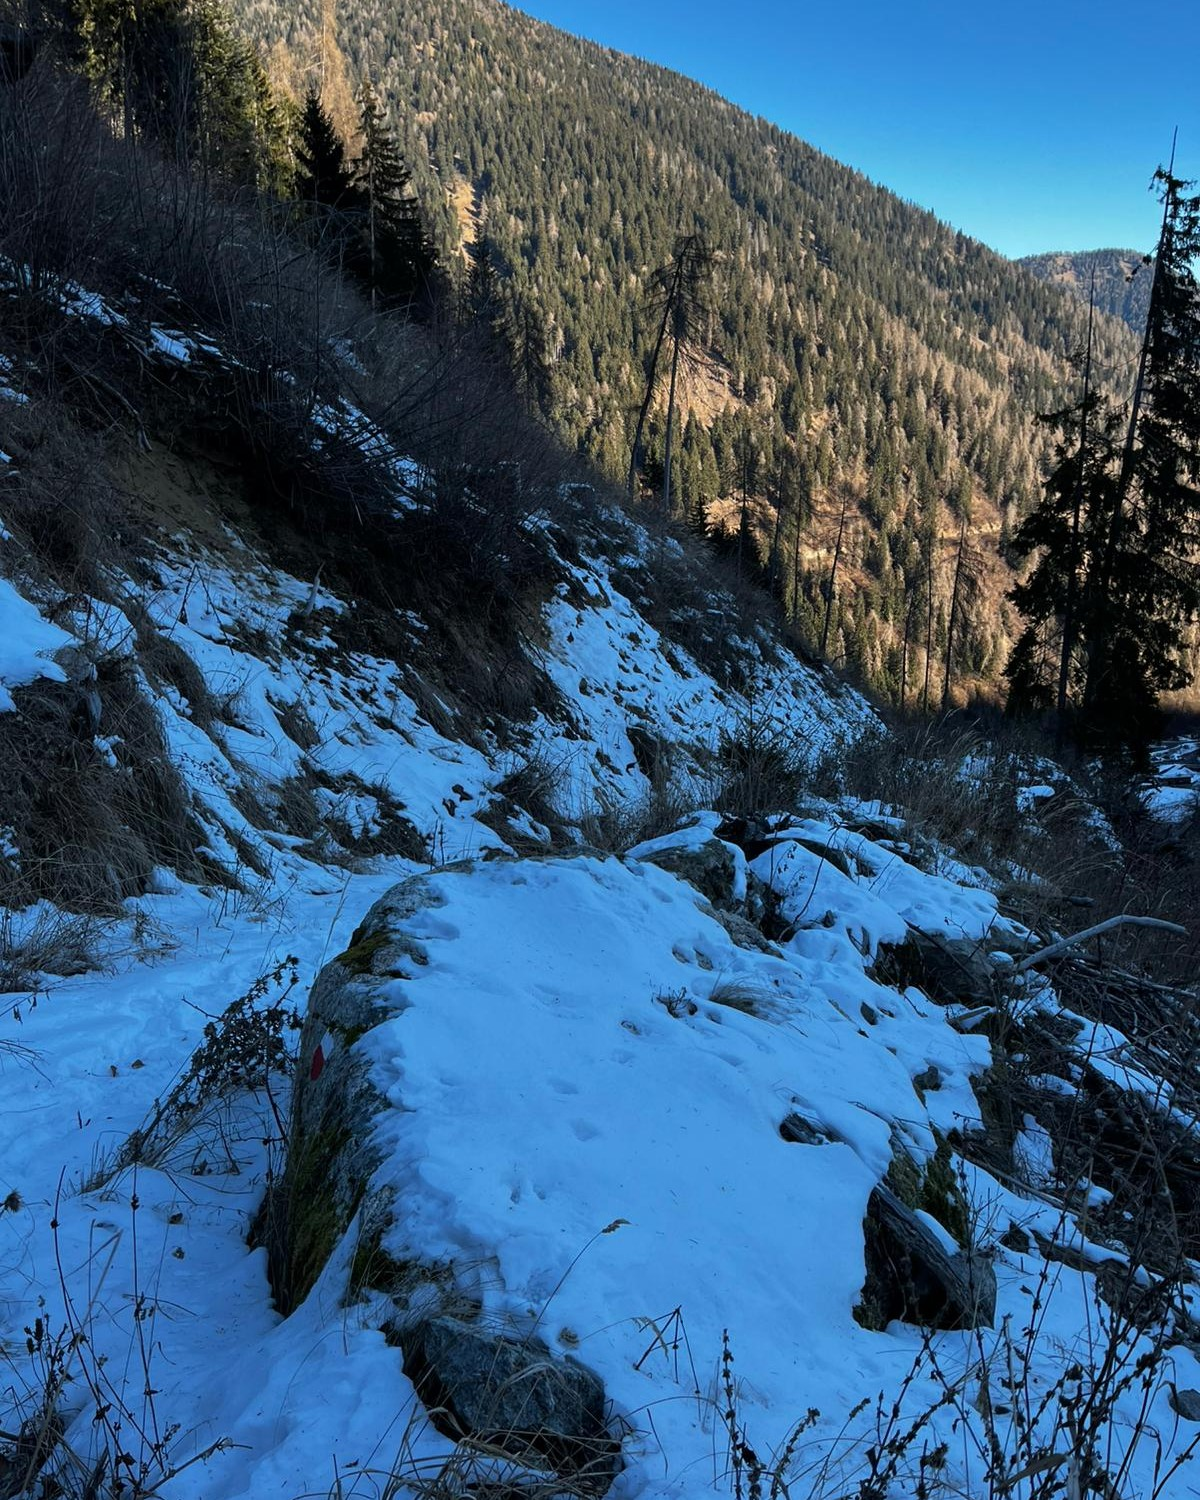
\includegraphics[width=\linewidth]{images/foto_sentiero.jpg}
        \caption{Sentiero.}
        \label{fig:foto2}
    \end{subfigure}
    
    \vspace{2em} 
    
    % Seconda riga: Altre due foto affiancate
    \begin{subfigure}{0.45\textwidth}
        \centering
        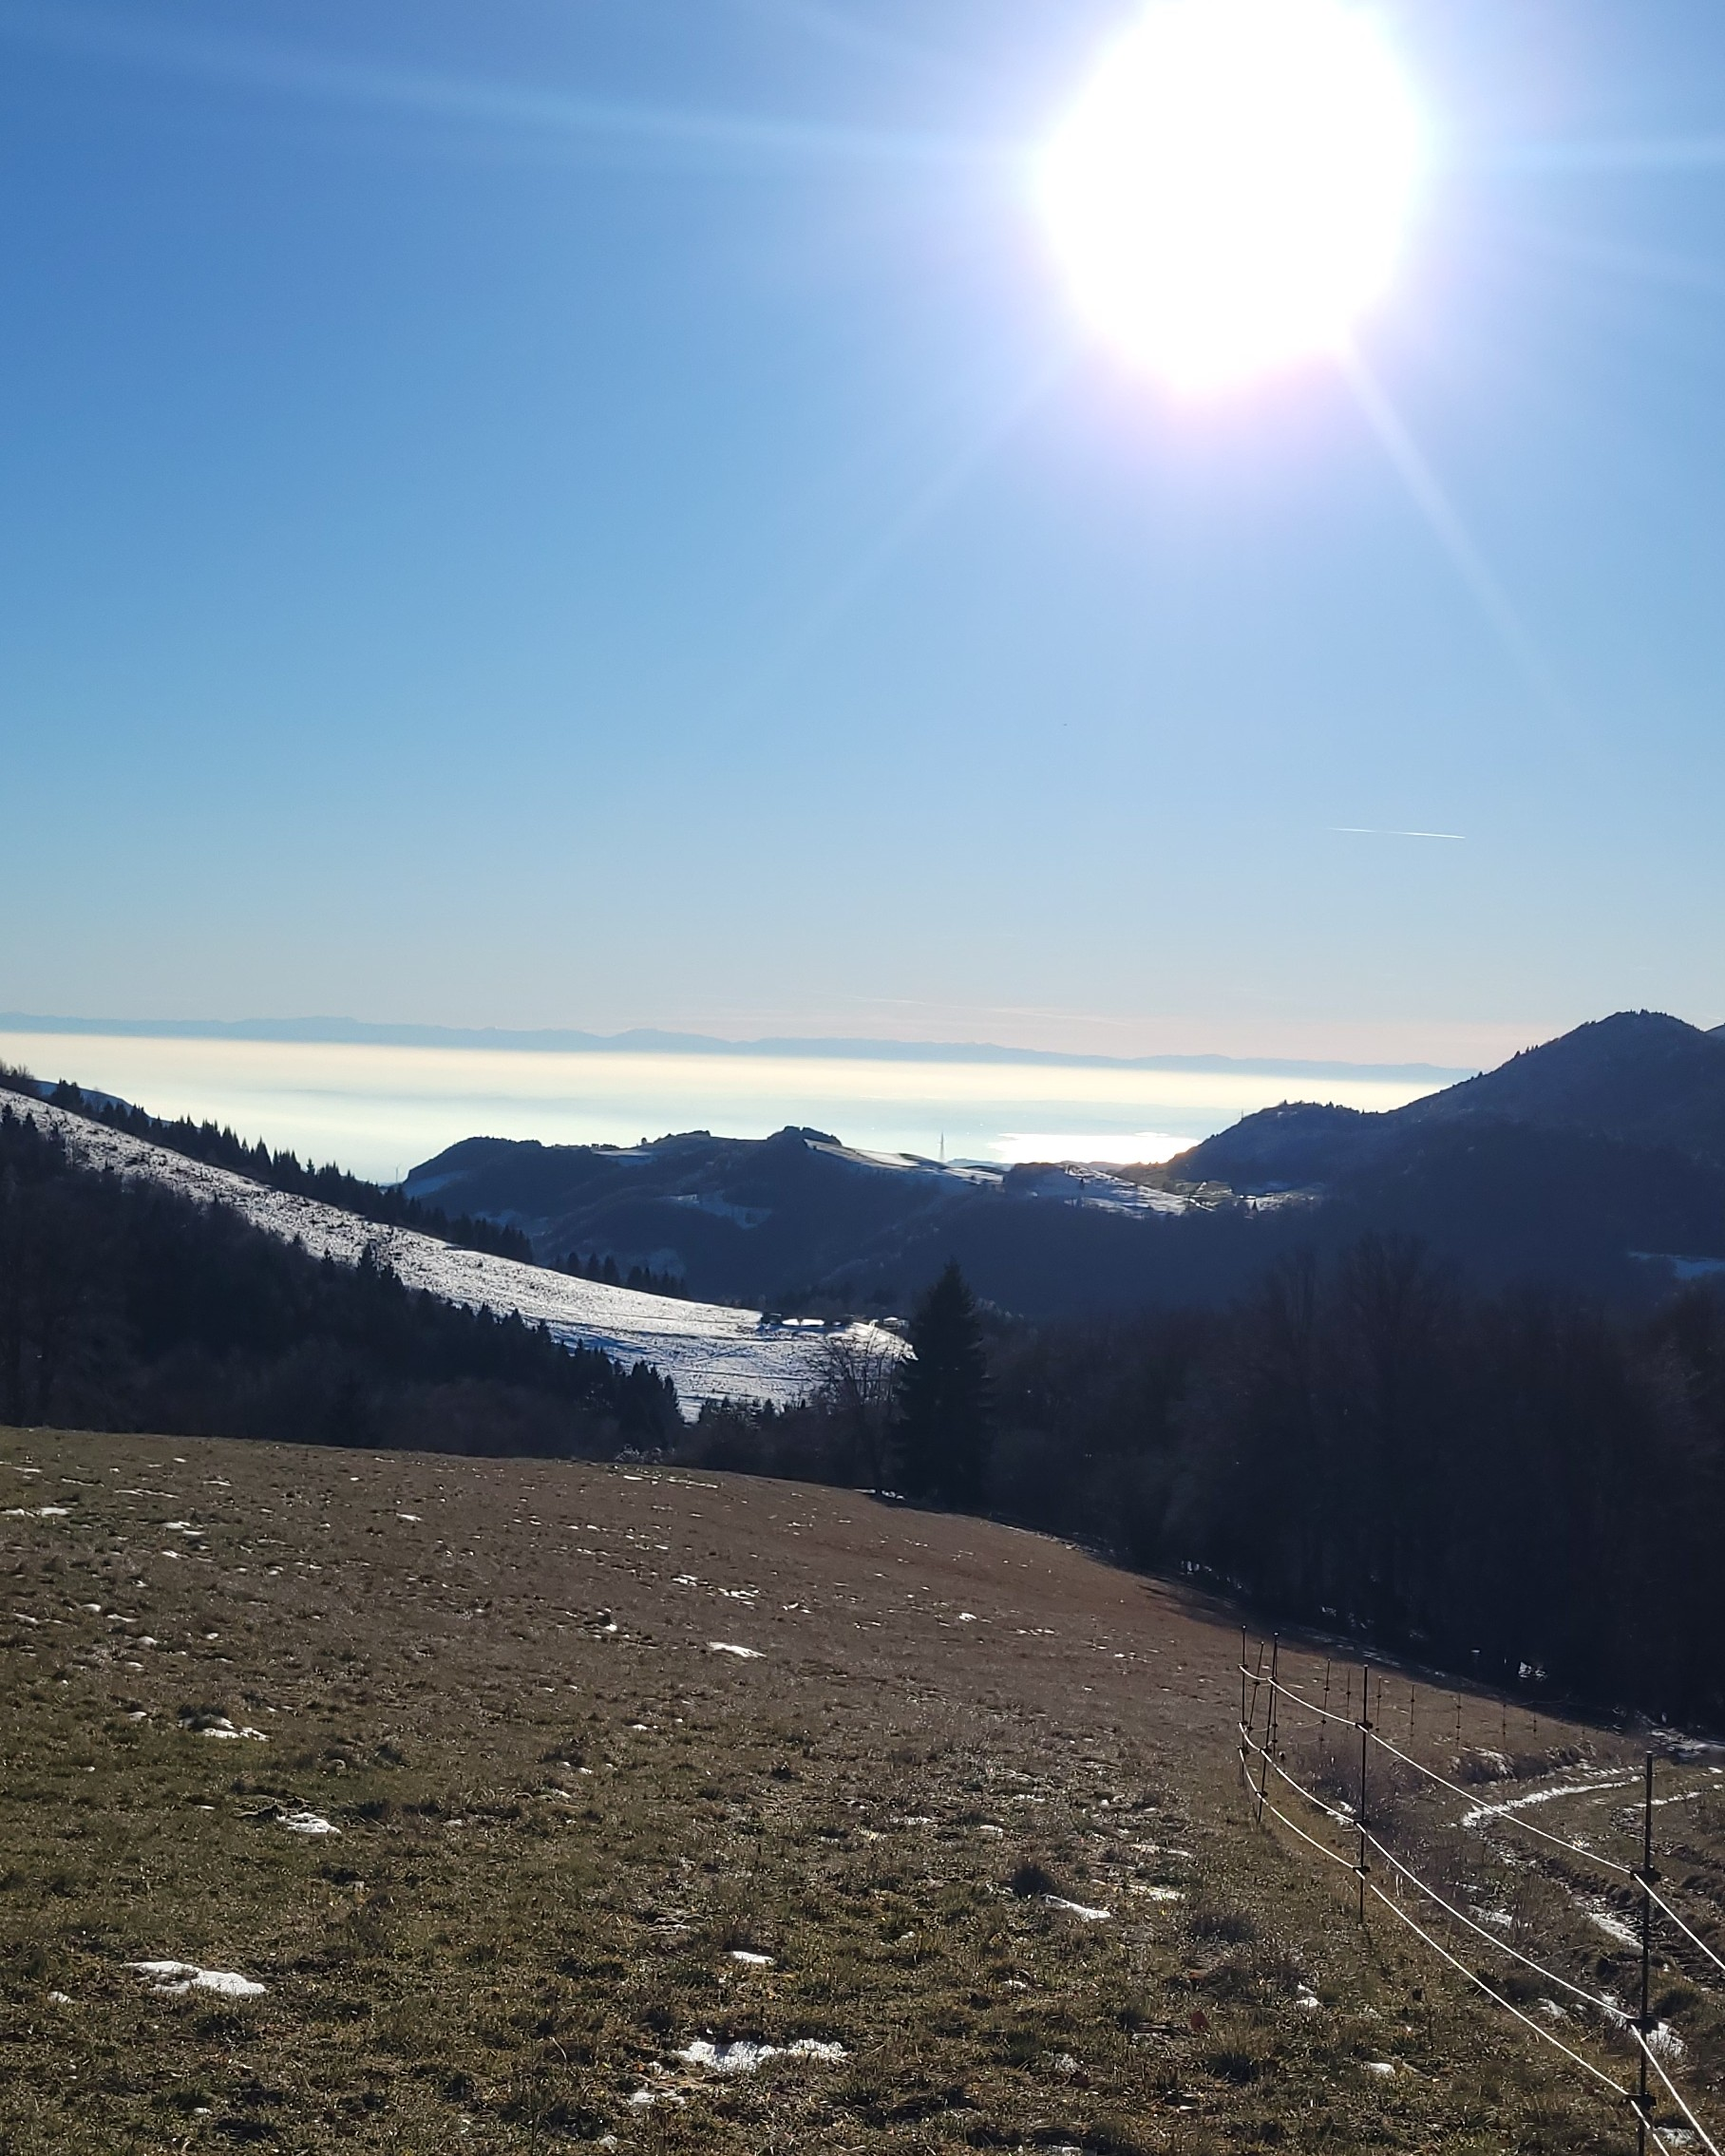
\includegraphics[width=\linewidth]{images/foto_paesaggio.jpg}
        \caption{Paesaggio.}
        \label{fig:foto3}
    \end{subfigure}
    \hfill 
    \begin{subfigure}{0.45\textwidth}
        \centering
        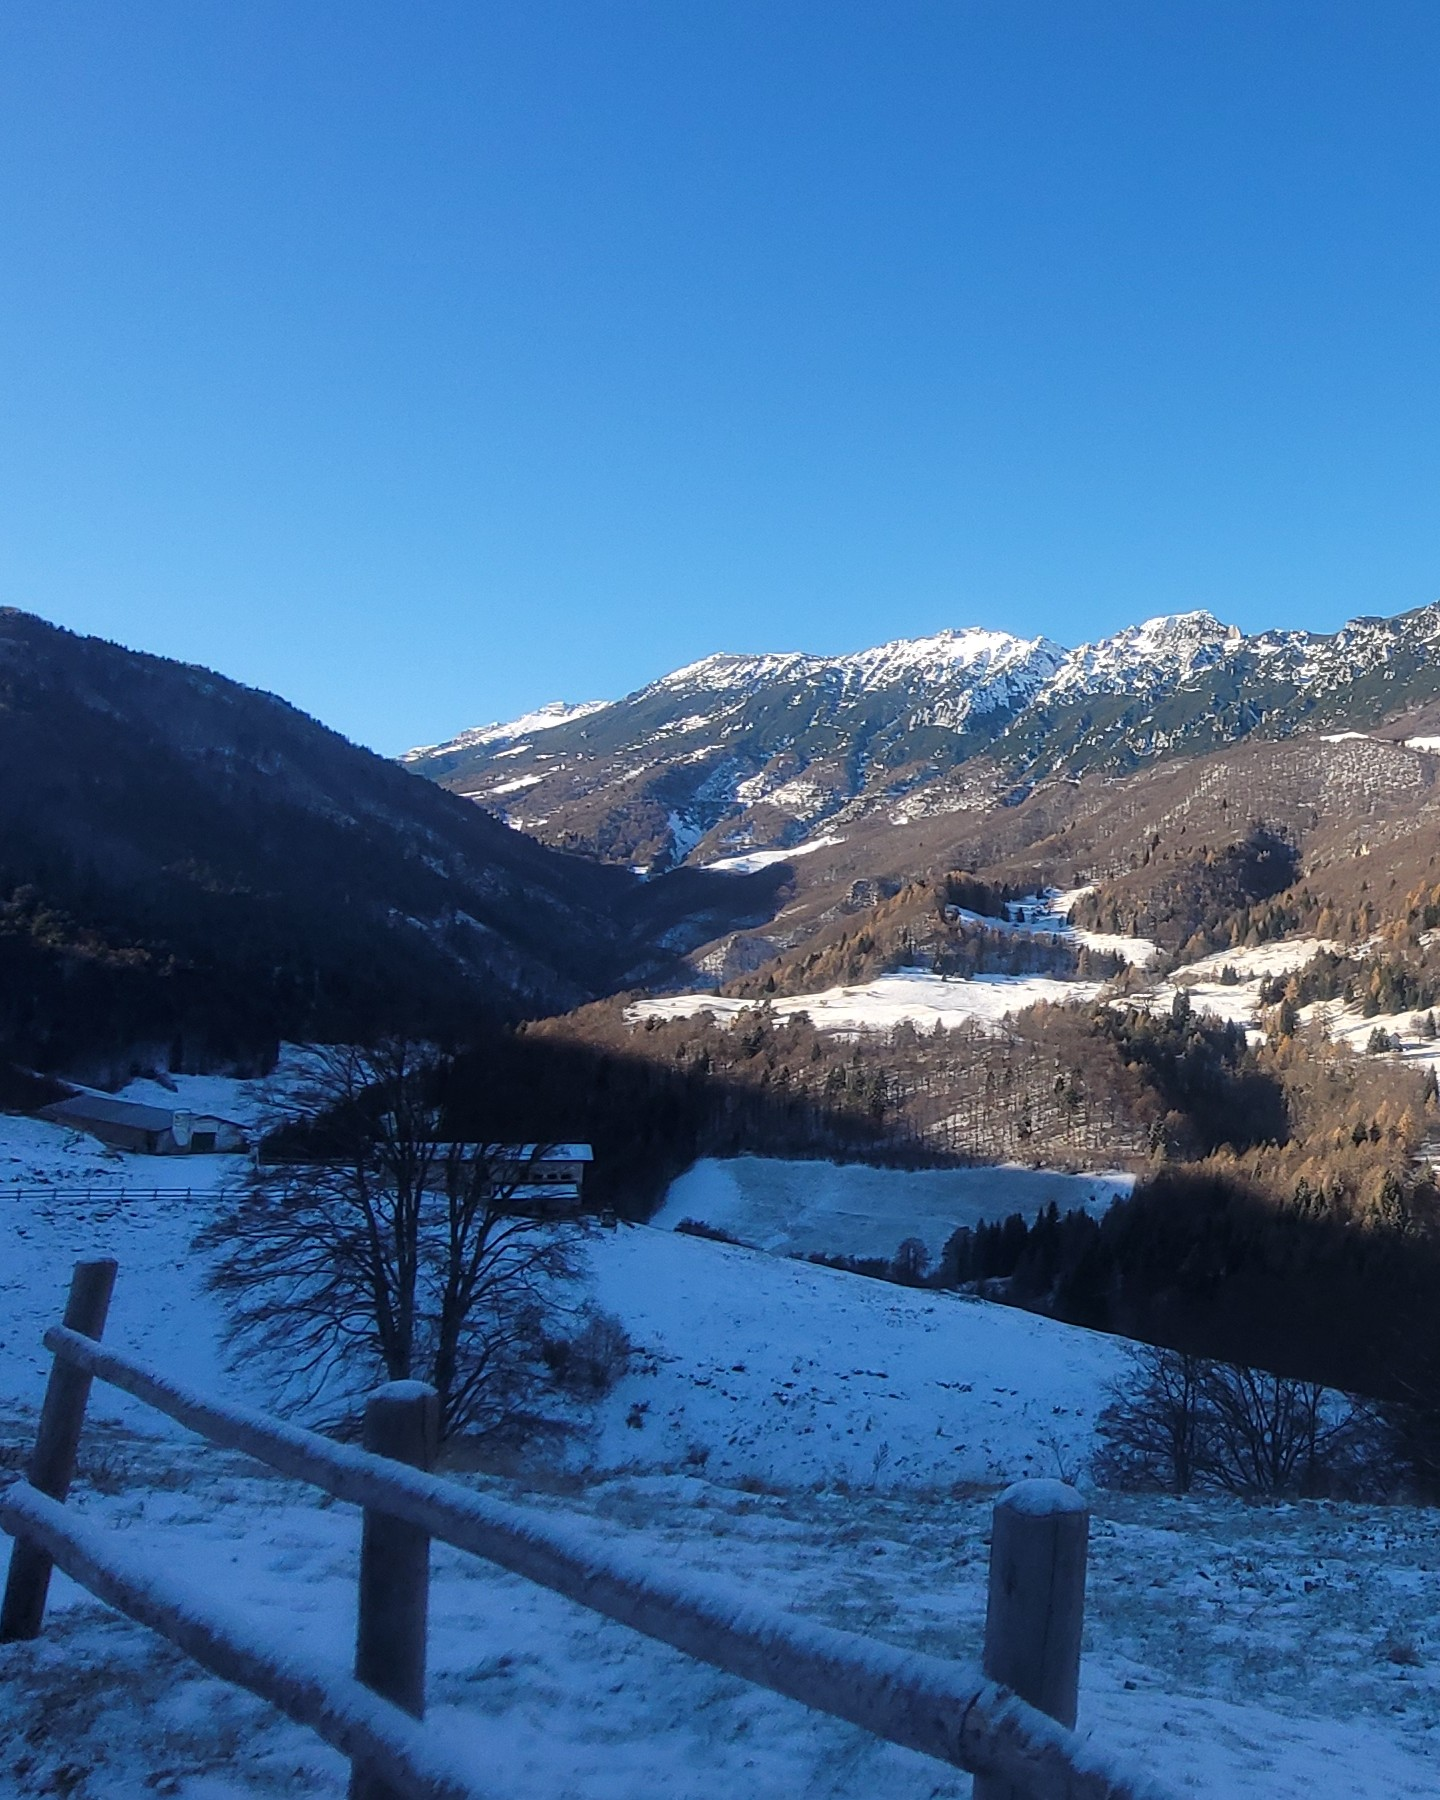
\includegraphics[width=\linewidth]{images/foto_vistaBivacco.jpg}
        \caption{Vista dal bivacco.}
        \label{fig:foto4}
    \end{subfigure}

    \caption{Selezione di fotografie del percorso e della vista dal bivacco.}
    \label{fig:panoramica_4_foto}
\end{figure}

\end{document}
